\chapter{Who is Fatigued? Examining Officer Attitudes Towards PWUOs, Naloxone, and Their Role in Responding to Opioid Overdoses}

\section{Introduction}

The opioid overdose crisis, one of the longest ongoing public health crises, worsened in recent years when opioid overdose fatalities eclipsed 80,000 \parencite{center_for_disease_control_and_prevention_national_2023}. Since the 1990s a host of policies and programs have been implemented to reduce opioid overdose fatalities. One of the most common state-level policies of the last couple decades has been the implementation of Naloxone Access Laws (NALs). Naloxone is an opioid antagonist that binds to opioid receptors blocking the opioid from latching to the receptors \parencite{lurigio_opioid_2018}. This allows for the individual experiencing the overdose to regain proper respiratory functioning. According to the Legislative Analysis and Public Policy Association (LAPPA), every state has some form of a NAL, although the components of the policy varies \parencite{legislative_analysis_and_public_policy_association_naloxone_2022}. Additionally, Good Samaritan Laws (GSLs) have been signed into law in 50 states (and D.C.) which generally provide immunity to those who overdose as well as those who aid in helping the individual who overdosed, although the language varies from state to state \parencite{west_good_2023}. With the expansion of naloxone accessibility and the medication's ability to reverse opioid overdoses, as well as the immunity provided by GSLs, police departments have been increasingly outfitting their officers with naloxone \parencite{lurigio_opioid_2018}. In addition to carrying naloxone, there been efforts to act on police officers' frequent interactions with people who use drugs (PWUDs) and have them involved in collaborative efforts with social outreach organizations to reduce opioid overdose fatalities \parencite{donnelly_law_2022, formica_characteristics_2021, yatsco_alternatives_2020}. There is empirical evidence that suggests outfitting officers with naloxone can reduce overdose fatalities \parencite{rando_intranasal_2015}. Likewise, collaborative approaches between police department and public health agencies have been found to be effective at reducing fatal opioid overdoses \parencite{donnelly_law_2022} although the empirical base is limited given this is a relatively new approach.

However, while police officers have generally positive views of naloxone, some research has found that officers develop negative attitudes towards PWUDs, people who use opioids (PWUOs), naloxone, and drug treatment modalities as they respond to more overdoses \parencite{carroll_knowledge_2020, murphy_police_2020, murphy_police_2021}. This has been described as a potential compassion fatigue effect, where officers lose empathy and develop negative attitudes after repeatedly being involved in traumatic incidents \parencite{figley_compassion_1995, figley_treating_2002}. Compassion fatigue is not confined to police work and has been highlighted across professional contexts \parencite{adams_compassion_2006}. Within the police context, the development of negative attitudes with increased overdose response has implications for their involvement in opioid related issues. If officers develop negative attitudes their support for treatment may subside and there is the potential that it produces more punitive responses, which could hinder any collaborative or public health focused approach towards drug use \parencite{winstanley_bell_2020}.

In this study I explore Tempe police officer's perceptions and attitudes towards naloxone, PWUDs/PWUOs, and their role in responding to opioid overdoses across multiple waves of surveys. Then, I examine the relationship between opioid overdose response frequency and officer's perceptions. The findings have implications for police involvement in opioid overdose responses and police training focused substance use, and PWUOs.

\section{Literature Review}
\subsection{Police attitudes towards naloxone and PWUDs}
The police have increasingly become involved in responding to opioid overdoses and administering naloxone to combat rising opioid overdose fatalities. In some cases, the police are involved in referral or diversion programs to meet opioid overdose survivors with the potential to engage with social services. Due to law enforcement frequently being the first point of contact for someone who overdoses and a shift towards a public health model in some localities \parencite{beletsky_police_2011, silverman_harmonizing_2012}, there is a potential for police officers to save lives and to act as a conduit to services. While officer attitudes towards these issues were unexplored previously, their increased role in the opioid overdose crisis has prompted research into this area.

Prior work has found that officers have generally favorable attitudes towards naloxone and their role in responding to overdoses \parencite{purviance_law_2017, wagner_training_2016, white_narcan_2021}. Officers have reported feeling a sense of helplessness on scene at an overdose without being equipped with naloxone \parencite{banta-green_police_2013, white_moving_2021}. One way to improve officers’ ability to effectively handle an overdose situation is to provide them with naloxone. In 2013, Deputy Director of the U.S. National Drug Control Policy emphasized the importance of law enforcement to carry naloxone \parencite{michael_botticelli_announcing_2013}. Additionally, The Bureau of Justice Assistance highlighted that in addition to the ability to save lives, naloxone provides an improvement to job satisfaction among police officers \parencite{bureau_of_justice_assistance_law_nodate}. Indeed, outfitting officers with a medication that reverses the effects of an overdose is generally viewed favorably among officers. Having naloxone is another tool to use in order to save someone's life \parencite{lloyd_its_2023}. Other research has noted that the police want to be able to effectively provide life-saving care to reverse the effects of an overdose indicating their desire to carrying naloxone \parencite{purviance_law_2017}. And the idea of collaboration with public health agencies to address drug use is viewed as a more effective approach than traditional methods in some jurisdictions \parencite{lloyd_its_2023}.

Police officers can effectively administer naloxone and are receptive to training \parencite{lloyd_its_2023, pourtaher_naloxone_2022, purviance_law_2017, wagner_training_2016}. Police officers have displayed confidence in handling overdose situations as well \parencite{purviance_law_2017, ray_police_2015}. \textcite{white_narcan_2021} show that the items measuring competence and confidence had statistically significant improvements between wave 1 and wave 2 surveys (e.g., prior to carrying naloxone and 6 months after). Officers reported that they were more likely to disagree that they needed more training, that they were concerned about making a mistake, and that they were fearful of being sued. Officers were more likely to agree that they can recognize signs of an overdose, able to deal effectively with an overdose, and able to perform the recovery position on an overdose victim. Other studies have also found that competence tends to improve following training modules or experience with naloxone \parencite{wagner_training_2016} 

In addition to confidence in handling opioid overdoses, police officers have displayed improved perceptions of risk compensation beliefs. Risk compensation beliefs refer to the idea that naloxone availability will be associated with riskier drug use because naloxone acts as a safety net and prevents fatal overdoses. For instance, a recent study indicates that officers believed that naloxone and syringe exchange programs can lead to further opioid use \parencite{reichert_police_2023}. In a separate study, \textcite{winograd_concerns_2019} show that following a training, police officers' risk compensation beliefs improved significantly, which suggests these perceptions may be malleable.

Other research has casted doubt on the role of the police as a collaborative entity in combating the opioid overdose crisis \parencite{carroll_police_2023}. Police officers are not immune from stigmatizing views of PWUOs. While officers may have generally positive views of naloxone and their role in saving lives, much like the general population they still have negative perceptions towards PWUOs \parencite{barry_stigma_2014, calabrese_opposition_2019}. Studies have found that officers tend to agree that those who overdose are to blame \parencite{beletsky_attitudes_2005, wagner_training_2016}, naloxone enables PWUOs to continue using \parencite{banta-green_police_2013, burris_stopping_2009, reichert_police_2023}, and that naloxone encourages riskier drug use \parencite{saunders_you_2019}. Some of the negative perceptions can be corrected through training \parencite{winograd_concerns_2019}. Though others have shown that some perceptions may be less amenable following training modules \parencite{wagner_training_2016}. Additionally, law enforcement involvement in overdose situations can lead to criminalizing PWUOs \parencite{lowder_twoyear_2020, van_der_meulen_thats_2021}. Criminalization is not only harmful for the overdose victim but can subsequently lead to a hesitancy to call 911 due to fear of a police response and potential arrest \parencite{bohnert_policing_2011}. If police officers are often the first point of contact for PWUOs, their attitudes towards PWUOs, and their perceived role in the opioid overdose crisis is an important consideration. The development of negative perceptions and/or attitudes towards PWUOs could influence their discretion at the scene of an overdose resulting in more punitive outcomes for PWUOs.

\subsection{Compassion fatigue}

In addition to general attitudes towards naloxone, PWUOs, and officers’ role in responding to opioid overdoses, previous work has found that with increased response to opioid overdoses officers’ attitudes towards naloxone PWUOs decline. This is suggestive of a compassion fatigue effect. Compassion fatigue refers to the negative effect of vicarious traumatization. That is, an individual in an occupation where they care for and interact with individuals who experience traumatic events (e.g., first responders, therapists, etc.) may be vicariously traumatized and over time may become less empathetic and develop pessimistic attitudes \parencite{adams_compassion_2006, figley_compassion_1995}. 

While qualitative work has highlighted this potential compassion fatigue effect among police officers and other first-responders \parencite{banta-green_police_2013, saunders_you_2019}, more recent work has explored this finding quantitatively. \textcite{carroll_knowledge_2020} finds that as the frequency of overdose response increases, attitudes towards their scale of ‘enforcement overdose response efforts’ decline. Specifically, those who reported responding more than 4 times per month to an overdose has a composite score of 6.84. For those who had not responded to an overdose, their composite score was 8.13 which indicates a higher level of agreement towards law enforcement overdose response efforts. 

Likewise, \textcite{murphy_police_2020} investigate the compassion fatigue hypothesis using both bivariate and multivariate analyses for a sample of police officers in Pennsylvania. Murphy and Russell’s findings support the notion that officers feel trained and want to be involved in responding to opioid overdoses. Yet, they find that officers have negative attitudes towards drug treatment and PWUDs and that these negative attitudes are related to frequency of overdose response and naloxone administrations. \textcite{murphy_police_2021} also find that increased overdose response and naloxone administrations were negatively associated with treatment oriented policies.

\section{Current Study}

I am interested in examining how officers’ attitudes have changed towards naloxone, their role in responding to opioid overdoses, and PWUOs over four waves of surveys. This broad interest is driven by the compassion fatigue literature that suggests officer attitudes may become more pessimistic, less empathetic, and less supportive of overdose response efforts as they respond to more opioid overdoses. To evaluate the compassion fatigue hypothesis, I investigate two research questions:

1) Are officers’ attitudes towards naloxone, their role in responding to opioid overdoses, and their perceptions of PWUOs changing over time? 

\begin{flushleft}
\(H1_a\): Officer's attitudes towards their role in responding to opioid overdoses, naloxone, and PWUOs will change over time.
\end{flushleft}

2) Is opioid overdose response frequency associated with officer attitudes towards their role in responding to opioid overdoses, naloxone, and PWUOs? 

\begin{flushleft}
\(H2_a\): Officer's attitudes towards naloxone, PWUOs, and their role in responding to opioid overdoses will have a relationship with opioid overdose response frequency.
\end{flushleft}

To answer these research questions, I use survey data that captures Tempe officers’ attitudes at different time points over a four-year period. To examine attitudinal change over time, I will employ unconditional linear growth models. To answer the second research question, I run pooled OLS regression models with wave fixed effects to explore how the frequency of opioid overdose response impacts officers’ attitudes.

\section{Methods}
\subsection{Setting}

Since 2020 the Tempe Police Department (TPD) has been involved in a collaborative effort with a social services organization – EMPACT – to reduce opioid overdose fatalities in Tempe, Arizona. This project, called the Tempe First-Responder Opioid Recovery Project, is funded by the Substance Abuse and Mental Health Services Administration (SAMHSA). The project trained and outfitted Tempe officers with naloxone in January of 2020 and created a 24/7 crisis hotline which officers contacted following an overdose incident to get in contact with a peer navigator (e.g., social outreach worker). Within days of the incident the peer navigator meets with the overdose survivor and their family/friends to provide information regarding potentially useful services (e.g., counseling, drug rehabilitation, housing information, transportation, etc.). Tempe officers have responded to more than 300 overdose incidents during the project. They have administered naloxone over 250 times in which it aided in a successful reversal of opioid overdose symptoms, and they have contacted the 24/7 crisis hotline approximately the same number of times. 

\subsection{Data}

The data for this study come from multiple waves of surveys administered throughout the duration of the Tempe ORP. The first wave of surveys was administered prior to the project in December of 2019 (n = 242). In October of 2020, the second wave of surveys was administered (n = 117). These two waves were the focus of our prior study looking at officers’ perceptions \parencite{white_narcan_2021}. The third wave was conducted in November of 2021 (n = 62) and the final wave was administered in March and April of 2023 (n = 109). The first three waves of surveys were administered electronically through Google Forms. Due to the decline in the response rate in wave 3, hard copy surveys were used for the fourth wave to improve our response rate.  I attended 10 patrol briefings with the project manager at TPD and handed out hard copy surveys to a total of 18 squads (111 officers). All four waves of surveys were voluntary and anonymous. The survey took approximately 12 to 15 minutes both electronically and hard copy. The surveys mostly comprised of true/false and Likert scale statements that are on a four-point scale (1 = strongly disagree, 4 = strongly agree). Additionally, all four surveys utilize the OOKS and OOAS scales \parencite{williams_development_2013} and the NaRRC-B scale \parencite{winograd_concerns_2019}. The survey also captured officer demographics.

\subsection{Dependent Variables}

I focus on three mean index measures: The role of the police,  naloxone related beliefs, and stigma towards PWUOs (see Appendix B.1 for more detail). The role of the police is captured by indexing four items, "I am glad to be carrying naloxone," "Tempe police officers should carry naloxone," "I feel better able to do my job carrying naloxone," and "Police should not respond to overdoses."\footnote{Police should not respond to overdoses is reverse coded.} The items produce a Cronbach's alpha that is above the conventional .70 threshold (\(\alpha = .774\)).

Naloxone related compensation beliefs is captured with five items, "People will use more if they have access to naloxone," "Users will be less likely to go to treatment due to naloxone," "Limit the number of naloxone administrations per person," "Naloxone enables PWUDs to continue their use," and "Providing naloxone means I condone opioid use." These items produce a Cronbach's alpha that is above the conventional .70 threshold (\(\alpha = .868\)).

To measure stigma towards PWUOs I index four items, "People who overdose need to learn a lesson," "People who overdose deserve life-threatening outcomes," "People who overdose are to blame," and "Overdose survivors should be arrested." The items produce a Cronbach's alpha that is just below the conventional threshold of .70 (\(\alpha = .692\)).

The reasons these measures are chosen as outcome variables are two-fold. First, these items measure the concepts of interest and are of particular importance if they do indeed change over time or are influenced by opioid overdose response frequency. Theoretically, compassion fatigue would impact officer's attitudes towards these items. For instance, a decline in empathy towards PWUOs may produce pessimistic attitudes towards this population. Secondly, prior work on this topic has used similar measures. \textcite{murphy_police_2020} use a few different items. To capture officer attitudes towards naloxone they provide the following statements in their survey instrument: “Increasing access and utilization of Narcan is a good solution to the opioid problem,” “Increasing access and utilization of Narcan provides individuals with a substance use disorder an excuse to continue their drug use,” and “There should be a limit on how often someone who overdoses be administered Narcan.” While \textcite{carroll_knowledge_2020} use a “OD response efforts scale” that contains five Likert scale items that correspond to a variety of overdose prevention efforts such as distribution of naloxone, the value of Good Samaritan Laws, and community based prevention training programs. Following both \textcite{murphy_police_2020} and \textcite{carroll_knowledge_2020}, I use similar outcome variables that may be influenced by compassion fatigue. 

\subsection{Independent Variable}

There are two primary independent variables in this study. For the first research question, the wave of the survey is the independent variable of interest (i.e., 1, 2, 3, 4). The wave of the survey is effectively a measure of time which allows for an examination of how time is associated with shifts in attitudes. For the second research question, opioid overdose response frequency is the independent variable of interest. This variable is measured on a five-point scale: “Never (0),” “Rarely (less than once per week) (1),” “Once per week (2),” “Once per shift (3),” and “Multiple times per shift (4).”

Control variables include whether the respondent is a patrol officer; reference category is non-patrol. Having ever administered naloxone is measured as a dummy variable. Sex is measured as a dummy variable; males are the reference category. Race is captured as Black, Hispanic, and Other, while the reference category is White non-Hispanic. Education is measured as a dummy variable that indicates if the respondent has received a college education which includes two-year, four-year, and advanced degrees; the reference category includes high school diploma or a GED, and some college. Time spent at the Tempe Police Department is represented as a series of dummy variables 1-2 years, 3-5 years, 6-10 years, 11+ years at the department; the reference category is less than one year at the department. I then control for competence at the scene of an overdose. This variable is measured on a four-point Likert scale from completely disagree (1) to completely agree (4). Specifically, this item states “I would be able to effectively deal with an overdose.” A dummy variable for having administered naloxone is included in the model as well. Lastly, I incorporate wave fixed effects to control for unobservable time invariant characteristics between the waves of the survey.

\subsection{Analytical Sample}

The final analytical sample is comprised of 527 observations. However, listwise deletion removes approximately 13\% of the sample in the pooled ordinary least squares (OLS) regression models.\footnote{Models 1 and 3 drop 62 observations (13\%), Model 2 drops 61 observations (12\%).} 

Tables 1 and 2 provide a breakdown of the sample descriptive statistics. I will focus on table 2 here to discuss the descriptive statistics across the waves.\footnote{Because the fourth survey was administered in-person at roll-call, the sample in the fourth wave is younger and more likely to be on patrol compared to the first three waves. I control for both of these variables in the main regression models and run sensitivity checks on a patrol only sample (see Appendix B.3).} Focusing on the independent variable, frequency of overdose response increased across the waves. Never having responded to an overdose declined from wave 1 (19\%) to wave 4 (7\%) while responding to an overdose once per week increased by approximately 8\%. The most common response across all four waves is less than once per week (40\%-47\%). Ever having administered naloxone increased across the waves from 2\% to 67\%. Additionally, respondents are predominately White (70\%-89\%), male (81\%-87\%), college educated (67\%-83\%), and have been at the Tempe Police Department for 11 or more years (32\%-70\%).

\subsection{Analytical Plan}

The analysis proceeds as follows. First, to descriptively examine the change in attitudes over time, I will use three unconditional linear growth models. These will provide estimates for how attitudes have changed across the multiple waves of surveys over the course of the project. Then, to examine the relationship between opioid overdose response frequency and officer attitudes, I run three pooled OLS regression models with wave fixed effects.

\subsubsection{Unconditional Linear Growth Models}

\[Y_t = \beta_0 + \beta_1 Wave_t + \epsilon_t \]

Where \(Y_t\) is the outcome of interest (Police role, stigma towards PWUOs, and naloxone related beliefs) at wave \(t\). \(\beta_0\) is the intercept of outcome \(Y\). \(\beta_1\) is the coefficient for the primary independent variable -- waves of the survey. This represents the change in \(Y\) across the waves. Error is captured with the \(\epsilon_t\) term.

\subsubsection{Pooled OLS Regression Models}

\[Y = \beta_0 + \beta_1 OD response frequency + \beta_n X_n + \alpha_t + \epsilon \]

Where \(Y\) is the outcome of interest (Police role, stigma towards PWUOs, and naloxone related beliefs). \(\beta_0\) is the intercept of outcome \(Y\). \(\beta_1\) is the coefficient for the primary independent variable -- opioid overdose response frequency. \(\beta_n X_n\) represents the coefficients for a vector of covariates described above. \(\alpha_t\) represents wave fixed effects for wave \(t\). Error is captured with \(\epsilon\).

\section{Results}

Table 3 provides the results from the unconditional linear growth models. The results suggest that the wave of the survey is associated with changes in attitudes towards \textit{the role of the police} and \textit{stigma towards PWUOs}. Compared to wave 1, there was an increase of .152 (\(p < .1\)) in wave 3 and an increase of .372 (\(p < .01\)) in wave 4 for officer's support for their role in responding to opioid overdoses. Additionally, compared to wave 1, there was an increase of .249 (\(p < .01\)) in wave 3 and an increase of .155 (\(p < .05\)) in wave 4 for stigmatizing perceptions of PWUOs. Although these estimates are statistically significant, their standardized coefficients represent relatively small changes over time.\footnote{\textit{The role of the police} wave 3 standardized \(\beta\) = .08; wave 4 standardized \(\beta\) = .24. \textit{Stigma towards PWUOs} wave 3 standardized \(\beta\) = .14; wave 4 standardized \(\beta\) = .11.} Figure 1 provides a visualization of the unstandardized estimates across the waves of surveys. 

Table 4 presents the coefficients for the pooled OLS regression models. Here, I will restrict my discussion of the results by focusing on the primary independent variable of interest \parencite{keele_causal_2020}. The primary independent variable - opioid overdose response frequency - is not associated with any of the outcomes of interest. I will discuss this finding and other variables' relationships in more detail below. 

\section{Discussion}

In the present study I investigate the compassion fatigue hypothesis within the context of police responding to opioid overdoses using two approaches. First, the unconditional linear growth models provide mixed support for the first hypothesis. Officers' perceptions of \textit{the role of the police} and \textit{stigma towards PWUOs} did change over time. \textit{Perceptions of naloxone} did not change over time. Like previous work in this area, police officers generally had a positive view of naloxone and their role in saving lives \parencite{white_narcan_2021, pourtaher_naloxone_2022, reichert_police_2023}. The increased support for their role in responding to opioid overdoses may be related to the effectiveness of naloxone \parencite{white_leveraging_2022} or the effective working relationship with EMPACT, a social service organization who engages in post-overdose outreach with officers from the department \parencite{white_moving_2021}. Interestingly, the largest increase in officer attitudes towards their role in responding to overdoses is accompanied by a compositional change in the sample for wave 4. Respondents in this wave are younger, less likely to have a college degree, and more likely to be a patrol officer. Thus, they are most likely to be responding to opioid overdoses. Other work has demonstrated negative relationships between these covariates and officer attitudes towards opioid related issues \parencite{kruis_police_2020, reichert_police_2023}.

On the other hand, \textit{stigma of PWUOs} increases over time. Although data limitations prevent me from exploring this finding further, it is worth mentioning that over the course of the project the percentage of individuals who were homeless and received naloxone from Tempe police officers increased from 13\% in year one to 45\% in the final year of the project. The extent to which this trend contributed to an increase in stigmatizing views of PWUOs is unknown but there is evidence to suggest that officers who view PWUOs as unemployed or from a lower social class may perceive them to be more dangerous \parencite{kruis_police_2020}.

Second, I examine the relationship between opioid overdose response frequency and officer perceptions. Opioid overdose response frequency was not associated with any of the outcomes of interest. This suggests that opioid overdose exposure was not associated with improved or diminished attitudes towards the police role, naloxone, or stigma towards PWUOs. This finding holds true in a sensitivity check on a patrol only sample as well (see Appendix B.3). This finding runs counter to prior work that has reported an association between opioid response frequency and increased negative attitudes/perceptions \parencite{carroll_knowledge_2020, murphy_police_2020, murphy_police_2021}. It may be the case that Tempe officers have bought in to the role of responding to overdoses and administering naloxone. Prior to the first survey Tempe police officers did not have naloxone. \textcite{white_moving_2021} show that some officers felt a sense of futility when on scene at an overdose without naloxone, similar to studies in other jurisdictions, which has been found in other jurisdictions \parencite{smiley-mcdonald_perspectives_2022}. Having naloxone may be viewed as a tool that officers are able to quickly and easily use to save lives \parencite{lloyd_its_2023}. 

There were some covariate associations that are worth mentioning. Ever having administered naloxone was associated with an increase in support for officers' role in responding to opioid overdoses. Additionally, females were less likely to develop negative attitudes towards PWUOs. Similar to the analysis of the first two waves of surveys \parencite{white_narcan_2021}, those with a college degree and those who had been at the department longer (2-5, 6-10, and 11+ years) had negative attitudes towards the police role in opioid overdoses. These findings are counter to some of the findings in prior work, particularly for education \parencite{jorgensen_badges_2018}. Lastly, those who had higher levels of competence in handling an overdose were more likely to endorse the police role in opioid overdoses but also developed negative attitudes towards PWUOs. 

\subsection{Limitations}
The present study offers an analysis of the perspectives of Tempe police officers over the span of approximately 4 years. However, there are limitations that should be discussed. First, these attitudes are likely not generalizable to other jurisdictions. The Tempe Police Department is known for its focus on evidence-based practices. Over the last decade, they have participated in multiple research projects, including two randomized controlled trials (evaluating body-worn cameras and de-escalation training). The generally positive views from the first two ORP survey waves may be a product of the culture at Tempe PD \parencite{white_narcan_2021}. Second, the last wave of data used in the analysis come from in-person, hard copy administered surveys that were completed in tandem with “Narcan life-saving awards” being handed out by the project manager at Tempe PD. The first two survey waves were administered online. The context surrounding the administration of the final wave of surveys could increase the chance of social desirability impacting officers’ responses. Because the project manager, the awards, and I were present, this could have prompted the officers to respond more positively to survey items. However, whether this occurred or to what extent is unknown. Third, the between-subjects design of this study only examines aggregate mean trends across waves. While this approach is informative, it is limiting in that I am unable to measure within-subject variance over time. Future studies that examine the compassion fatigue hypothesis should attempt to overcome this limitation by creating a panel dataset of officer attitudes. Lastly, an aspect of officers' perceptions that is not available for modeling in this chapter is where the officer is patrolling. It may be the case that certain characteristics of neighborhoods or beats impact officers' perceptions of PWUOs, naloxone, and their role in the opioid overdose crisis. Future research should investigate the role of place in influencing officer perceptions related to the opioid crisis. 

\subsection{Implications}
Some potential implications can be gleaned from the findings. On a practical note, for program implementation and sustainability, patrol-level officer buy-in is an essential ingredient to a successful program. In order to facilitate this buy-in, broad department culture and immediate supervisor perceptions of these issues is also likely to be an important factor \parencite{del_pozo_police_2024}. Tempe Police Department had an internal champion guiding training's and garnering support within the department. This could be a contributing factor to officers' positive views and increased agreement towards their role in responding to opioid overdoses over time. 

Additionally, updated training modules for officers that cover substance use and naloxone is likely to play an important role. Training's have been shown to combat opioid myths surrounding fentanyl \parencite{del_pozo_can_2021}. This could also be applied to improving officer perceptions of PWUOs, particularly concerning stigmatizing views \parencite{winograd_concerns_2019}. If stigmatizing perceptions are associated with an increase in punitive outcomes, more harm will be created \parencite{binswanger_clinical_2016, ray_spatiotemporal_2023} and public-health approach to getting PWUOs in contact with potentially useful services will be hindered. The importance of training's and immediate supervisors are quite relevant here \parencite{del_pozo_police_2024}.  

\section{Conclusion}

The increased level of agreement with respect to the police role in opioid overdoses is likely due to a variety of factors including department culture, the effectiveness of naloxone, and the collaborative relationship between TPD and EMPACT \parencite{white_narcan_2021, white_moving_2021}. Tempe officers seem to buy-in to their role of carrying and administering naloxone. Regarding the increased stigma towards PWUOs, reintroducing training's focused on substance use should be offered to officers to provide more information related to opioids, naloxone, and PWUOs. 


\pagebreak
% table headers
% descriptive stats
\begin{table}[htbp]\centering
\def\sym#1{\ifmmode^{#1}\else\(^{#1}\)\fi}
\caption{\centering Summary Statistics}
\begin{tabular}{l*{1}{cccc}}
\toprule
                &     Mean&       SD&      Min&      Max\\
\midrule
\emph{Dependent Variables}&         &         &         &         \\
Role of the police&     2.98&     0.63&     1.00&     4.00\\
Naloxone related beliefs&     2.21&     0.56&     1.00&     4.00\\
Stigma towards PWUOs&     2.38&     0.59&     1.00&     4.00\\
\emph{OD Response Frequency}&         &         &         &         \\
Never           &     0.15&     0.36&     0.00&     1.00\\
Rarely (less than once per week)&     0.45&     0.50&     0.00&     1.00\\
Once per week   &     0.32&     0.47&     0.00&     1.00\\
Once per shift  &     0.05&     0.22&     0.00&     1.00\\
Multiple times per shift&     0.02&     0.13&     0.00&     1.00\\
\vspace{0.1em} \emph{Control Variables}&         &         &         &         \\
Ever administered naloxone&     0.25&     0.43&     0.00&     1.00\\
Patrol          &     0.57&     0.50&     0.00&     1.00\\
Female          &     0.16&     0.37&     0.00&     1.00\\
White           &     0.77&     0.42&     0.00&     1.00\\
Black           &     0.04&     0.19&     0.00&     1.00\\
Hispanic        &     0.14&     0.35&     0.00&     1.00\\
Other           &     0.05&     0.21&     0.00&     1.00\\
College degree  &     0.77&     0.42&     0.00&     1.00\\
Competence at an overdose&     2.94&     0.79&     1.00&     4.00\\
\emp{Time at Tempe PD}&         &         &         &         \\
Less than 1 year&     0.05&     0.22&     0.00&     1.00\\
1-2 years       &     0.07&     0.26&     0.00&     1.00\\
2-5 years       &     0.15&     0.36&     0.00&     1.00\\
6-10 years      &     0.15&     0.36&     0.00&     1.00\\
11+ years       &     0.58&     0.49&     0.00&     1.00\\
\bottomrule
\multicolumn{5}{l}{\footnotesize n = 527}\\
\end{tabular}
\end{table}


% descriptive stats by wave
% fix sd space in wave 4
\begin{landscape}
\begin{table}[htbp]\centering
\def\sym#1{\ifmmode^{#1}\else\(^{#1}\)\fi}
\caption{\centering Summary Statistics by Wave}
\begin{tabular}{l*{4}{cc}}
\hline\hline
                &        1&         &        2&         &        3&         &        4&         \\
\hline
\emph{Dependent Variables}&         &         &         &         &         &         &         &         \\
\hspace{0.25cm} Role of the police&     2.87&   (0.63)&     2.97&   (0.57)&     3.02&   (0.74)&     3.24&   (0.53)\\
\hspace{0.25cm} Naloxone related beliefs&     2.18&   (0.55)&     2.23&   (0.60)&     2.21&   (0.64)&     2.23&   (0.50)\\
\hspace{0.25cm} Stigma towards PWUOs&     2.30&   (0.56)&     2.39&   (0.60)&     2.55&   (0.62)&     2.45&   (0.60)\\
\emph{OD Response Frequency}&         &         &         &         &         &         &         &         \\
\hspace{0.25cm} Never&     0.19&   (0.39)&     0.17&   (0.38)&     0.13&   (0.34)&     0.07&   (0.26)\\
\hspace{0.25cm} Rarely (less than once per week)&     0.47&   (0.50)&     0.43&   (0.50)&     0.40&   (0.49)&     0.47&   (0.50)\\
\hspace{0.25cm} Once per week&     0.29&   (0.45)&     0.32&   (0.47)&     0.39&   (0.49)&     0.37&   (0.49)\\
\hspace{0.25cm} Once per shift&     0.04&   (0.19)&     0.07&   (0.25)&     0.06&   (0.25)&     0.06&   (0.23)\\
\hspace{0.25cm} Multiple times per shift&     0.01&   (0.11)&     0.02&   (0.13)&     0.02&   (0.13)&     0.03&   (0.17)\\
\vspace{0.1em} \emph{Control Variables}&         &         &         &         &         &         &         &         \\
\hspace{0.25cm} Ever administered naloxone&     0.02&   (0.14)&     0.22&   (0.41)&     0.45&   (0.50)&     0.67&   (0.47)\\
\hspace{0.25cm} Patrol&     0.47&   (0.50)&     0.53&   (0.50)&     0.53&   (0.50)&     0.85&   (0.36)\\
\hspace{0.25cm} Female&     0.16&   (0.37)&     0.14&   (0.34)&     0.18&   (0.38)&     0.19&   (0.39)\\
\hspace{0.25cm} White&     0.78&   (0.41)&     0.75&   (0.44)&     0.89&   (0.31)&     0.70&   (0.46)\\
\hspace{0.25cm} Black&     0.04&   (0.19)&     0.03&   (0.17)&     0.00&   (0.00)&     0.07&   (0.26)\\
\hspace{0.25cm} Hispanic&     0.13&   (0.34)&     0.17&   (0.37)&     0.07&   (0.26)&     0.18&   (0.38)\\
\hspace{0.25cm} Other&     0.05&   (0.21)&     0.06&   (0.23)&     0.04&   (0.19)&     0.05&   (0.22)\\
\hspace{0.25cm} College degree&     0.79&   (0.41)&     0.80&   (0.40)&     0.82&   (0.38)&     0.67&   (0.47)\\
\hspace{0.25cm} Competence at an overdose&     2.48&   (0.72)&     3.10&   (0.66)&     3.40&   (0.61)&     3.51&   (0.52)\\
\emp{Time at Tempe PD}&         &         &         &         &         &         &         &         \\
\hspace{0.25cm} Less than 1 year&     0.04&   (0.20)&     0.01&   (0.09)&     0.00&   (0.00)&     0.14&   (0.34)\\
\hspace{0.25cm} 1-2 years&     0.07&   (0.25)&     0.04&   (0.20)&     0.03&   (0.18)&     0.14&   (0.34)\\
\hspace{0.25cm} 2-5 years&     0.17&   (0.38)&     0.13&   (0.34)&     0.03&   (0.18)&     0.20&   (0.40)\\
\hspace{0.25cm} 6-10 years&     0.12&   (0.32)&     0.11&   (0.32)&     0.25&   (0.44)&     0.20&   (0.40)\\
\hspace{0.25cm} 11+ years&     0.60&   (0.49)&     0.70&   (0.46)&     0.68&   (0.47)&     0.32&   (0.47)\\
\hline\hline
\multicolumn{9}{l}{\footnotesize Mean, Standard deviation in parentheses; Wave 1 (n = 239), Wave 2 (n = 117), Wave 3 (n = 62), Wave 4 (n = 109)}\\
\end{tabular}
\end{table}

\end{landscape}


% growth model figure
% fix to include the note as the image note not the graph note
\begin{figure}
    \centering
    \caption{\centering Unconditional Linear Growth Models}
    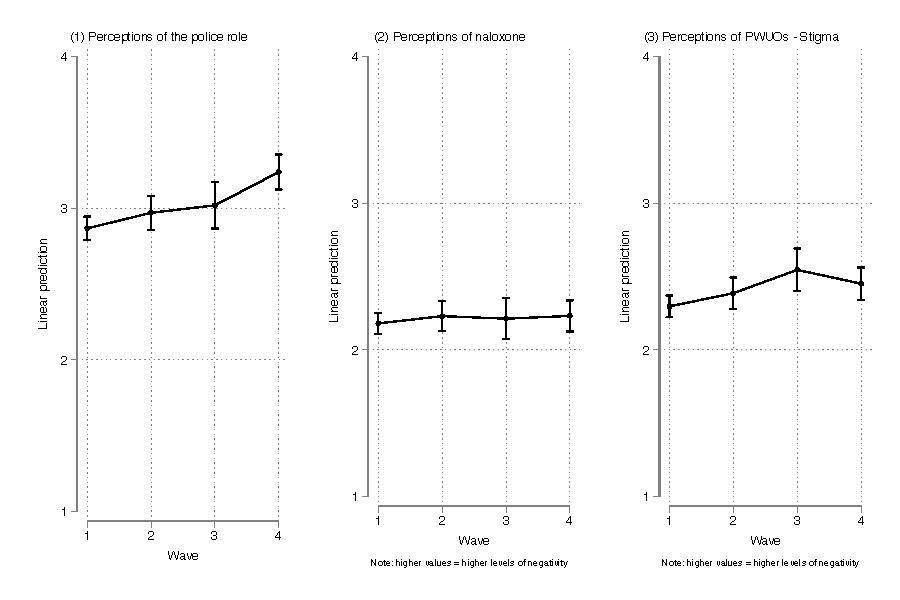
\includegraphics{figures/growth_models.pdf}
\end{figure}

% growth model coefficients table
\begin{table}[htbp]\centering
\def\sym#1{\ifmmode^{#1}\else\(^{#1}\)\fi}
\caption{\centering Unconditional Linear Growth Models}
\begin{tabular}{l*{3}{c}}
\toprule
                &\multicolumn{1}{c}{(1)}&\multicolumn{1}{c}{(2)}&\multicolumn{1}{c}{(3)}\\
                &\multicolumn{1}{c}{Role of the police}&\multicolumn{1}{c}{Naloxone related beliefs}&\multicolumn{1}{c}{Stigma towards PWUOs}\\
\midrule
Wave 2          &0.103 (0.069)        &0.050 (0.063)        &0.090 (0.066)        \\
\addlinespace
Wave 3          &0.152\sym{+} (0.087)        &0.032 (0.080)        &0.249\sym{**} (0.083)        \\
\addlinespace
Wave 4          &0.372\sym{**} (0.071)        &0.051 (0.065)        &0.155\sym{*} (0.067)        \\
\addlinespace
Constant        &2.867\sym{**} (0.040)        &2.181\sym{**} (0.036)        &2.297\sym{**} (0.038)        \\
\midrule
Observations    &      527        &      525        &      527        \\
\bottomrule
\multicolumn{4}{l}{\footnotesize Standard errors in parentheses}\\
\multicolumn{4}{l}{\footnotesize \sym{+} \(p<0.10\), \sym{*} \(p<0.05\), \sym{**} \(p<0.01\)}\\
\end{tabular}
\end{table}


% pooled reg models coefficients
% add note re robust se's in model (1) + reference categories: never responding to an overdose, never administered naloxone, White, male, less than a year at the department, in wave 1.
\begin{landscape}
   \begin{table}[htbp]\centering
\def\sym#1{\ifmmode^{#1}\else\(^{#1}\)\fi}
\caption{\centering Pooled OLS Regression Models}
\begin{tabular}{l*{3}{c}}
\toprule
                &\multicolumn{1}{c}{(1)}&\multicolumn{1}{c}{(2)}&\multicolumn{1}{c}{(3)}\\
                &\multicolumn{1}{c}{\hspace{0.25cm} Role of the police}&\multicolumn{1}{c}{\hspace{0.25cm} Naloxone related beliefs}&\multicolumn{1}{c}{\hspace{0.25cm} Stigma towards PWUOs}\\
\midrule
\emph{OD Response Frequency}&                  &                  &                  \\
\hspace{0.25cm} Rarely (less than once per week)&0.024 (0.082)         &-0.076 (0.076)         &-0.101 (0.078)         \\
\hspace{0.25cm} Once per week&0.000 (0.091)         &-0.005 (0.088)         &-0.069 (0.091)         \\
\hspace{0.25cm} Once per shift&0.034 (0.167)         &0.010 (0.133)         &-0.113 (0.138)         \\
\hspace{0.25cm} Multiple times per shift&-0.246 (0.262)         &0.042 (0.206)         &-0.008 (0.213)         \\
\vspace{0.1em} \emph{Control Variables}&                  &                  &                  \\
\hspace{0.25cm} Ever administered naloxone&0.190\sym{***} (0.068)         &-0.094 (0.076)         &-0.035 (0.078)         \\
\hspace{0.25cm} Patrol&-0.095 (0.066)         &0.081 (0.061)         &0.034 (0.063)         \\
\hspace{0.25cm} Black&0.220 (0.134)         &0.040 (0.134)         &-0.134 (0.139)         \\
\hspace{0.25cm} Hispanic&-0.001 (0.070)         &0.119 (0.073)         &-0.009 (0.075)         \\
\hspace{0.25cm} Other&-0.059 (0.119)         &0.096 (0.121)         &0.079 (0.125)         \\
\hspace{0.25cm} Female&0.070 (0.075)         &0.072 (0.069)         &-0.158\sym{**} (0.072)         \\
\hspace{0.25cm} College degree&-0.173\sym{***} (0.062)         &-0.054 (0.061)         &-0.030 (0.063)         \\
\hspace{0.25cm} Competence at an overdose&0.172\sym{***} (0.053)         &-0.042 (0.040)         &0.099\sym{**} (0.041)         \\
\emp{Time at Tempe PD}&                  &                  &                  \\
\hspace{0.25cm} 1-2 years&-0.137 (0.103)         &0.180 (0.145)         &-0.026 (0.150)         \\
\hspace{0.25cm} 2-5 years&-0.240\sym{**} (0.115)         &0.199 (0.133)         &0.001 (0.138)         \\
\hspace{0.25cm} 6-10 years&-0.419\sym{***} (0.114)         &0.303\sym{**} (0.133)         &0.028 (0.138)         \\
\hspace{0.25cm} 11+ years&-0.318\sym{***} (0.096)         &0.114 (0.121)         &-0.040 (0.125)         \\
\emp{Wave}      &                  &                  &                  \\
\hspace{0.25cm} Wave 2&0.012 (0.071)         &0.037 (0.070)         &0.053 (0.072)         \\
\hspace{0.25cm} Wave 3&0.046 (0.110)         &0.042 (0.094)         &0.119 (0.098)         \\
\hspace{0.25cm} Wave 4&0.051 (0.092)         &0.067 (0.090)         &0.066 (0.093)         \\
Constant        &2.901\sym{***} (0.179)         &2.130\sym{***} (0.164)         &2.153\sym{***} (0.170)         \\
\midrule
Observations    &      459         &      458         &      459         \\
\(R^{2}\)       &    0.164         &    0.050         &    0.051         \\
\bottomrule
\multicolumn{4}{l}{\footnotesize Standard errors in parentheses}\\
\multicolumn{4}{l}{\footnotesize \sym{*} \(p<0.10\), \sym{**} \(p<0.05\), \sym{***} \(p<0.01\)}\\
\end{tabular}
\end{table}
 
\end{landscape}

%Create appendix for tables of cronbach's alpha measurements on outcomes, linear growth model for patrol only 